% \newpage
\thispagestyle{empty}
\section{Решения контрольной работы 2}

\subsection[2017-2018]{\hyperref[sec:kr_02_2017_2018]{2017-2018}}
\label{sec:sol_kr_02_2017_2018}

\begin{enumerate}
\item[7.]
\begin{enumerate}
\item Всем хватит места, если число явившихся на рейс пассажиров ($X$) не превысит $300$,
то есть нужно найти $\P(X \leq 300)$. Найдём матожидание и дисперсию
случайной величины $X$:
\begin{align*}
\E(X) &= np = 330 \cdot 0.9 = 297 \\
\Var(X) &= np(1-p) = 330 \cdot 0.9 \cdot 0.1 = 29.7
\end{align*}
Теперь посчитаем нужную вероятность:
\[
\P(X \leq 300) = \P \left(\frac{X - 297}{\sqrt{29.7}} \leq \frac{300 - 297}{\sqrt{29.7}} \right) = \P(\cN(0,1) \leq 0.55) \approx 0.709
\]
\item Вероятность переполнения не должна превышать $0.1$:
\begin{align*}
&\P(X > 300) < 0.1 \\
&\P\left(\frac{X - 0.9 \cdot n}{\sqrt{0.9 \cdot 0.1 \cdot n}} > \frac{300 - 0.9 \cdot n}{\sqrt{0.9 \cdot 0.1 \cdot n}} \right) < 0.1 \\
&\frac{300 - 0.9 \cdot n}{\sqrt{0.9 \cdot 0.1 \cdot n}}  > 1.28 \\
&300 - 0.9n > 1.28 \cdot 0.3 \sqrt{n} \\
&n < 325.6
\end{align*}
\end{enumerate}
\item[8.]
\begin{enumerate}
\item Выпишем случайную величину $X_i$ — цену акции после $i$-ого дня:
\[
X_i =
\begin{cases}
1.01, & p = 0.7 \\
0.99, & p = 0.2999 \\
0, & p = 0.0001
\end{cases}
\]
Нужно посчитать ожидание цены акциии после 20 дней:
\[
\E(X_1 \cdot \ldots \cdot X_{20}) \stackrel{\text{незав-ть}}{=} \E(X_1) \cdot \ldots \cdot \E(X_{20}) = 1.004^{20} \approx 1.083
\]
\item По ЗБЧ:
\[
\plim_{n\to\infty} \frac{1}{n} \sum_{i=1}^n X_i = \E(X_i) = 1.004
\]
\item Аналогично пункту (а):
\[
\E(X_1 \cdot \ldots \cdot X_{n}) = (\E(X_1))^n = 1.004^n
\]
И понятно, что $1.004^n \to_{n\to\infty} +\infty$.
\item
\begin{align*}
\P(\text{разорения}) &= 1 - \P(X_1 > 0, \ldots, X_n >0) = 1 - \prod_{i=1}^n \P(X_i > 0) \\
&= 1 - (1 - 0.0001)^n \to_{n\to\infty} 1
\end{align*}
\end{enumerate}
\end{enumerate}




\subsection[2016-2017]{\hyperref[sec:kr_02_2016_2017]{2016-2017}}
\label{sec:sol_kr_02_2016_2017}

\begin{enumerate}
\item \begin{enumerate}
\item $\E (2\xi - \eta +1) = 2 \E (\xi) - \E (\eta) + 1 = 2\cdot 1 - (-2) + 1 = 5 $

$\Cov (\xi, \eta) = \E (\xi \eta) - \E(\xi) \E(\eta) = -1 - \cdot 1 \cdot (-2) = 1$

$\Corr (\xi, \eta) = \frac{\Cov(\xi, \eta)}{\sqrt[]{\Var(X) \cdot \Var(Y)}} = \frac{1}{\sqrt{1 \cdot (8-(-2)^2)}} = \frac{1}{2}$

$\Var (2\xi - \eta + 1) = 4\Var(\xi) + \Var(\eta) - 2 \Cov (2\xi, \eta) = 4 \cdot 1 + 4 - 4 \cdot 1 = 4$

\item $\Cov(\xi + \eta, \xi + 1) = \Cov(\xi) + \Cov(\xi, 1) + \Cov(\eta, \xi) + \Cov(\eta, 1) = 1 +1 = 2$

$\Corr(\xi + \eta , \xi + 1) = \frac{\Cov(\xi + \eta , \xi + 1)}{\sqrt{\Var(\xi + \eta)\cdot \Var (\xi + 1)}} = \frac{2}{\sqrt{(1+4+2\cdot 1) \cdot 1}} = \frac{2}{\sqrt{7}}$

$\Corr(\xi + \eta - 24, 365 - \xi - \eta) = -1$

$\Cov(2016\cdot \xi, 2017) = 0$

\end{enumerate}
\item
\begin{enumerate}
\item Частные распределения:

\begin{center}
\begin{tabular}{cccc}
\toprule
$x$ & $-1$ & $0$ & $2$ \\
$\P(\xi = x)$ & $0.3$ & $0.4$ & $0.3$ \\ \bottomrule
\end{tabular}
\hspace{1cm}
\begin{tabular}{ccc}
\toprule
$y$ & $-1$ & $1$ \\
$\P(\eta = y)$ & $0.5$ & $0.5$ \\ \bottomrule
\end{tabular}
\end{center}

$\E(\xi) = -1 \cdot 0.3 + 0 \cdot 0.4 + 2 \cdot 0.3 = 0.3$

$\E (\xi^2) = (-1)^2 \cdot 0.3 + 0^2 \cdot 0.4 + 2^2 \cdot 0.3 = 1.5$

$\Var(\xi) = \E(\xi^2) - (\E(\xi))^2 = 1.5 - 0.3^2 = 1.41$

$\E(\eta) = -1 \cdot 0.5 + 1 \cdot 0.5 = 0$

$\E(\eta^2) = (-1)^2 \cdot 0.5 + 1^2 \cdot 0.5 = 1$

$\Var(\eta) = \E(\eta^2)-(\E(\eta))^2 = 1 - 0^2 = 1$

\item
\begin{center}
\begin{tabular}{cccccc}
\toprule
$xy$ & $-2$ & $-1$ & $0$ & $1$ & $2$ \\
$\P(\xi \cdot \eta = xy)$ & $0.2$ & $0.2$ & $0.4$ & $0.1$ & $0.1$ \\ \bottomrule
\end{tabular}
\end{center}

$\E(\xi\cdot\eta) = (-2) \cdot 0.2 + (-1) \cdot 0.2 + 0 \cdot 0.4 + 1\cdot 0.1 + 2 \cdot 0.1 = -0.3$

$\Cov(\xi, \eta) = \E(\xi\cdot\eta) - \E(\xi)\cdot\E(\eta) = -0.3 - 0.3 \cdot 0 = -0.3$
\item Пусть случайная величина $X$ принимает значения $a_1, \ldots, a_m$, случайная веилчина $Y$ принимает значения $b_1, \ldots, b_n$. Тогда случйаня величина $X$ и $Y$ называются независимыми, если $\forall i=1, \ldots, m \quad \forall j=1, \ldots, n: \P(X = a_i \cap Y = b_j) = P(X = a_i) \cdot P(Y = b_j)$
\item Заметим, что $\P (\xi = -1 \cap \eta=-1)=0.1$, $\P(\xi=-1)=0.3$ и $\P(\eta=-1)=0.5$.

Тогда поскольку $\P (\xi = -1 \cap \eta=-1) \neq \P(\xi=-1) \cdot \P(\eta=-1)$, случайные величины $\xi$ и $\eta$ не являются независимыми.
\item $\P (\xi = -1 \cap \eta=1) = \frac{\P (\xi = -1 \cap \eta=1)}{\P(\eta=1)} = \frac{0.2}{0.5} = \frac{2}{5}$

$\P (\xi = 0 \cap \eta=1) = \frac{\P (\xi = 0 \cap \eta=1)}{\P(\eta=1)} = \frac{0.2}{0.5} = \frac{2}{5}$

$\P (\xi = 2 \cap \eta=1) = \frac{\P (\xi = 2 \cap \eta=1)}{\P(\eta=1)} = \frac{0.1}{0.5} = \frac{1}{5}$

Следовательно, условное распределение случайной величины $\xi$ при условии $\{\eta=1\}$ может быть описано следующей таблицей:

\begin{center}
\begin{tabular}{cccc}
\toprule
$x$ & $-1$ & $0$ & $2$ \\
$\P(\xi = x)$ & $2/5$ & $2/5$ & $1/5$ \\ \bottomrule
\end{tabular}
\end{center}

\item $\E(\xi \mid \eta = 1) = -1 \cdot \frac{2}{5} + 0 \cdot \frac{2}{5} + 2 \cdot \frac{1}{5} = 0$
\item $\E(\pi) = \E(0.5 \xi + 0.5 \eta) = 0.5 \E(\xi) + 0.5 \E(\eta) = 0.15$

\begin{align*}
\Var(\pi) &= \Var(0.5 \xi + 0.5 \eta) = \Var(0.5 \xi) + \Var(0.5\eta) + 2 \Cov (0.5\xi, 0.5\eta) \\
&= 0.25\Var(\xi) + 0.25\Var(\eta) + 2 \cdot 0.5 \cdot 0.5 \Cov(\xi, \eta) \\
&= 0.25 \cdot 1.41 + 0.25 \cdot 1 + 2 \cdot 0.5 \cdot 0.5 \cdot (-0.3) = 0.4525
\end{align*}
\item
\begin{align*}
\Var(\pi(\alpha)) &= \Var(\alpha \xi + (1-\alpha)\eta) = \alpha^2\Var(\xi) + (1-\alpha)^2 \Var(\eta) \\
&+ 2\alpha(1-\alpha) \Cov(\xi, \eta) = 1.41 \cdot \alpha^2 + 1\cdot (1-\alpha)^2 + 2\alpha(1-\alpha) \cdot (-0.3) \\
&= 1.41 \cdot \alpha^2 + (1-\alpha)^2 - 0.6 \cdot (\alpha - \alpha^2) \to \min_\alpha \\
\frac{\partial}{\partial \alpha} \Var(\pi(\alpha)) &= 2 \cdot 1.41 \cdot \alpha -2(1-\alpha) -0.6\cdot(1-2\alpha) \\
&= 2.82 \cdot \alpha - 2 + 2\alpha - 0.6 + 1.2 \cdot \alpha = 6.02 \cdot \alpha - 2.6 = 0 \\
\alpha &= \frac{2.6}{6.02} = 0.4319
\end{align*}
\end{enumerate}
\item \begin{enumerate}
\item Для любой неотрицательной случайной величины $X$ и любого числа $\lambda > 0$ справедлива оценка: $\P(X>\lambda) \leq \frac{\E(X)}{\lambda}$

Пусть случайная величина $\xi_i$ означает число посетителей сайта за $i$-ый день. По условию, $\xi_i \sim Pois(\lambda=250)$. Известно, что если $\xi \sim Pois(\lambda)$, то $\E(\xi) = \Var(\xi) = \lambda$.

Имеем:
\[
\P(\xi_i >500) \leq \P(\xi_i \geq 500) \leq \frac{\E(\xi_i)}{500} = \frac{250}{500} = \frac{1}{2}
\]
\item Для любой случайной величины $X$ с конечным $\E(X)$ и любого положительного числа $\epsilon > 0$ имеет место неравенство: $\P(X-\E(X)\geq\epsilon)\leq\frac{\Var(X)}{\epsilon^2}$

Обозначим $\bar{\xi}_n := \frac{1}{n} \left(\xi_1 + \ldots + \xi_n\right)$ – среднее число посетителей сайта за $n$ дней. Тогда
\[
\E\left(\bar{\xi}_n\right) = \E\left(\frac{1}{n} \sum_{i=1}^{n} \xi_i\right) = \frac{1}{n} \sum_{i=1}^{n} \E(\xi_i) = \frac{1}{n} \cdot n \cdot \lambda = \lambda = 250
\]
\[
\Var\left(\bar{\xi}_n\right) = \Var\left(\frac{1}{n} \sum_{i=1}^{n} \xi_i\right) = \frac{1}{n^2} \sum_{i=1}^{n} \Var (\xi_i) = \frac{n \cdot \lambda}{n^2} = \frac{\lambda}{n} = \frac{250}{n}
\]
Оценим вероятность
\[
\P\left(\left\vert\bar{\xi}_n-250\right\vert > 10\right) \leq \frac{\Var\left(\bar{\xi}_n\right)}{100} = \frac{250}{100\cdot n}
\]
Следовательно, $1 - \frac{250}{100\cdot n} \leq \P\left(\left\vert\bar{\xi}_n-250\right\vert \leq 10\right)$.

Найдём наименьшее целое $n$, при котором левая часть неравенства ограничена снизу $0.99 \leq 1 - \frac{250}{100\cdot n}$.

Имеем:
\[
0.99 \leq 1 - \frac{250}{100\cdot n} \Leftrightarrow \frac{250}{100\cdot n} \leq 0.01 \Leftrightarrow n \geq \frac{250}{100 \cdot 0.01} \Leftrightarrow n  \geq 250
\]
Значит, $n=250$ – наименьшее число дней, при котором с вероятностью не менее $99\%$ среднее число посетителей будет отличаться от $250$ не более чем на $10$.
\item  Требуется найти наименьшее целое $n$, при котором $\P\left(\left\vert\bar{\xi}_n-250\right\vert \leq 10\right) = 0.99$

Имеем:
\begin{align*}
&\P(\vert\bar{\xi}_n - 250\vert \leq 10) = 0.99 \Leftrightarrow \P(-10\leq \bar{\xi}_n - 250 \leq 10) = 0.99 \\
&\P(-10n \leq S_n - 250n \leq 10n) = 0.99 \\
&\E(S_n) = \E(\xi_1 + \ldots + \xi_n) = \E(\xi_1) + \ldots + \E(\xi_n) = 250 \cdot n\\
&\Var(S_n) = \Var(\xi_1 + \ldots + \xi_n) = \Var(\xi_1) + \ldots + \Var(\xi_n) = 250 \cdot n \\
&\P\left(\frac{-10n}{\sqrt{250n}} \leq \frac{S_n - \E (S_n)}{\sqrt{\Var(S_n)}} \leq \frac{10n}{\sqrt{250n}}\right) = 0.99  \\
&2 \Phi \left(\frac{10n}{\sqrt{250n}}\right) -1 = 0.99 \\
&\Phi \left(\frac{10n}{\sqrt{250n}}\right) = \frac{1 + 0.99}{2}  \\
&\frac{10n}{\sqrt{250n}} = 2.58 \\
&\sqrt{n} = 2.58 \cdot \frac{\sqrt{250}}{10}  \\
&n = 16.641
\end{align*}
Следовательно, наименьшее целое $n$, есть $n=17$.
\item Пусть $X_1, X_2, \ldots, X_n, \ldots$ – последовательность независимых случайных величин с одинаковыми конечными математическими ожиданимяи и фиксированными конечными дисперсиями. Тогда $\frac{X_1 + \ldots + X_n}{n} \stackrel{\P}{\to} \E(X_i)$ при $n \to \infty$.

В нашем случае случаные величины $\xi_1^2, \xi_2^2, \ldots, \xi_n^2, \ldots$ – независимы,

$\E(\xi_1^2) = \ldots = \E(\xi_n^2) = \ldots < + \infty$ и $\Var(\xi_1^2) = \ldots = \Var(\xi_n^2) = \ldots < + \infty$ . Поэтому в соответствии с ЗБЧ имеем:
\[
\frac{\xi_1^2 +\ldots+ \xi_n^2}{n} \stackrel{\P}{\to} \E(\xi_i^2) = \Var(\xi_i) +\E(\xi_i)^2 = \lambda + \lambda^2 = \lambda(\lambda+1) = 250\cdot251 = 62750
\]
\end{enumerate}

\item \begin{enumerate}
\item Пусть $X_1, X_2, \ldots, X_n, \ldots$ – последовательность независимых,
одинаково распределённых случайных величин с $0<\Var(X_i)<\infty$, $i \in \mathbb{N}$.
Тогда для любого (борелевского) множества $B \subseteq R$ имеет место
\[
\lim_{n \to \infty} \P\left(\frac{S_n - \E(S_n)}{\sqrt{\Var(S_n)}} \in B\right) = \int_B \frac{1}{\sqrt{2\pi}}e^{-t^2/2} dt,
\]
где $S_n := X_1, \ldots, X_n$, $n \in \mathbb{N}$

\item Введём случайную величину
\[
X_i = \begin{cases}
1, & \text{если на i-ом шаге Винни-Пух пошёл направо} \\
-1, & \text{если пошёл налево}
\end{cases}
\quad i=1,\ldots, n;
\]
Тогда $S_n := X_1 +\ldots+X_n$ означает местоположение Винни-Пуха в $n$-ую минуту его блужданий по прямой.

$\E(X_i) = -1 \cdot 1/2 + 1 \cdot 1/2 = 0$,

$\E(X_i^2) = (-1)^2 \cdot 1/2 + (1)^2 \cdot 1/2 = 1$,

$\Var(X_i) = \E(X_i^2) - \E(X_i)^2 = 1$,

$\E(S_n) = \E(X_1 + \ldots + X_n ) = \E(X_1) + \ldots + \E(X_n) = 0$,

$\Var(S_n) = \Var(X_1 + \ldots + X_n ) = \Var(X_1) + \ldots + \Var(X_n) = n$

\begin{align*}
\P(S_n \in (-\infty, -5]) &= \P(S_n \leq -5) = \P\left( \frac{S_n-\E(S_n)}{\sqrt{\Var(S_n)}} \leq \frac{-5-0}{\sqrt{n}} \right)  \\
&\stackrel{n=60}{=}\P\left( \frac{S_n-\E(S_n)}{\sqrt{\Var(S_n)}} \leq -0.6454\right) \approx \int_{-\infty}^{-0.6454} \frac{1}{\sqrt{2\pi}} e^{-t^2/2} dt \\
&= \Phi(-0.6454) = 1-\Phi(0.6454) \approx0.2593
\end{align*}
\item Для любых $n \in \mathbb{N}$ и всех $x \in \mathbb{R}$ имеет место оценка:
\[
\bigl|F_{S_n^{*}}(x) - \Phi(x)\bigr| \leq 0.48 \cdot \frac{\E(|\xi_i - \E\xi_i|^3)}{\Var^{3/2}(\xi_i)\cdot\sqrt{n}} \text{,}
\]
где $\Phi(x) = \int_{-\infty}^{x}\frac{1}{\sqrt{2\pi}}e^{-\frac{t^2}{2}}\,dt$, \; $S_n^* = \frac{S_n - \E(S_n)}{\sqrt{\Var(S_n)}}$, \; $S_n = \xi_1 + \ldots + \xi_n$

В нашем случае:
\[
\P\left( \frac{S_{60} - \E(S_{60})}{\sqrt{\Var(S_{60})}} \leq -0.6454 \right) = \P(S^*_{60} \leq -0.6454) =
F_{S^*_{60}} (-0.6454)
\]
Согласно неравенству Берри-Эссеена, погрешность $\vert F_{S^*_{60}} (-0.6454) - \Phi(-0.6454) \vert$ оценивается сверху величиной
\[
0.48 \cdot \frac{\E(\vert X_i - \E(X_i) \vert^3 )}{\Var(X_i)^{3/2} \cdot \sqrt{n}} = 0.48 \cdot \frac{\E(\vert X_i \vert^3)}{1\cdot\sqrt{60}} = \frac{0.48}{\sqrt{60}} \approx0.062
\]
\end{enumerate}
\item \begin{enumerate}
\item Сначала найдём плотность распределения случайной величины $X$.
Пусть $x \leq 0 $, тогда $f_X (X) = \int_{-\infty}^{+\infty} f_{X, Y} (x, y) dy  = 0$.

Пусть $x >0 $, тогда
\begin{align*}
f_X (X) &= \int_{-\infty}^{+\infty} f_{X, Y} (x, y) dy = \int_{0}^{+\infty} 0.005 e^{-0.05x-0.1y} dy \\
&= 0.005e^{-0.05x} \int_{0}^{+\infty} e^{-0.1y} dy = 0.005e^{-0.05x} \cdot \left(-10e^{-0.1y} \right) \bigg\vert_{y=0}^{y=+\infty} = 0.05 e^{-0.05x}
\end{align*}
Таким образом, имеем:
\[
f_X (x) = \begin{cases}
0.05 e^{-0.05x} & \text{при } x>0 \\
0 & \text{при } x \leq 0
\end{cases}
\]
То есть $X \sim Exp(\lambda=0.05)$ – случайная величина $X$ имеет показательное
распределение с параметром $\lambda = 0.05$.

Теперь найдём плотность распределения случайной величины $Y$.

Пусть $y \leq 0 $, тогда $f_Y (y) = \int_{-\infty}^{+\infty} f_{X, Y} (x, y) dx  = 0$.

Пусть $y > 0 $, тогда
\begin{align*}
f_Y (y) &= \int_{-\infty}^{+\infty} f_{X, Y} (x, y) dx  = \int_{0}^{+\infty} 0.005 e^{-0.05x-0.1y} dx \\
&= 0.005e^{-0.1y} \int_{0}^{+\infty} e^{-0.05x} dx = 0.005e^{-0.1y} \cdot \left(-20e^{-0.05x} \right) \bigg\vert_{x=0}^{x=+\infty} = 0.1 e^{-0.1y}
\end{align*}
Таким образом, имеем:
\[
f_Y (y) = \begin{cases}
0.1 e^{-0.1y} & \text{при } y>0 \\
0 & \text{при } y \leq 0
\end{cases}
\]
То есть $Y \sim Exp(\lambda=0.1)$ – случайная величина $Y$ имеет показательное распределение с параметром $\lambda = 0.1$.
\item Поскольку для любых точек $x, y \in \mathbb{R}$ справедливо равенство $f_{X, Y} (x, y) = f_X (x) \cdot f_Y (y)$, случайные величины $X$ и $Y$ являются независимыми.
\item Найдём вероятность $\P(Y>5)$:
\[
\P(Y>5) = \int_{5}^{+\infty} f_Y (y) dy = \int_{5}^{+\infty}  0.1 e^{-0.1y} dy = 0.1 \cdot (-10 e^{-0.1x}) \bigg\vert_{y=5}^{y=+\infty} = e^{-0.5} \approx0.6065
\]
\item Требуется найти условную вероятность $\P(Y>8 \mid Y \geq 3)$. Для этого предварительно найдём вероятности $\P(Y>8)$ и $\P(y \geq 3)$:
\[
\P(Y>8) = \int_{8}^{+\infty} f_Y (y) dy  = \int_{8}^{+\infty}  0.1 e^{-0.1y} dy = 0.1 \cdot (-10 e^{-0.1x}) \bigg\vert_{y=8}^{y=+\infty} = e^{-0.8}
\]
\[
\P(Y \geq 3) =  \int_{3}^{+\infty} f_Y (y) dy   =  \int_{3}^{+\infty}  0.1 e^{-0.1y} dy = 0.1 \cdot (-10 e^{-0.1x}) \bigg\vert_{y=3}^{y=+\infty} = e^{-0.3}
\]
Теперь находим требуемую условную веростность:
\[
\P(Y>8 \mid Y \geq 3) = \frac{\P(Y > 8 \cap
Y \geq 3)}{\P(Y \geq 3)} = \frac{\P(Y>8)}{\P(Y \geq 3) } = \frac{e^{-0.8}}{e^{-0.3}} = e^{-0.5} \approx0.6065
\]
\item Сначала найдём условную плотность распределения случайной величины $X$ при условии $Y=y$:
\begin{align*}
f_{X \mid Y} (x \mid y) &=
\begin{cases}
\frac{f_{X \mid Y} (x, y)}{f_Y (y)} & \text{при } f_Y (y) \\
0 & \text{иначе}
\end{cases} \\
&=
\begin{cases}
\frac{0.005e^{-0.05x-0.1y}}{0.1e^{-0.1y}} & \text{при } x>0, \quad y>0 \\
0 & \text{иначе}
\end{cases} \\
&= \begin{cases}
0.05 e^{-0.05x} & \text{при } x>0, \quad y>0 \\
0 & \text{иначе}
\end{cases}\\
&=
\begin{cases}
f_X (x) & \text{при } y > 0 \\
0 & \text{при } y \leq 0
\end{cases}
\end{align*}
Теперь находим условное математическое ожидание
\[
\E(X \mid Y=5) = \int_{-\infty}^{+\infty} xf_{X\mid Y} (x \mid 5) dx =  \int_{-\infty}^{+\infty} xf_{X} (x) dx = \E(X) = \frac{1}{0.05} =20
\]
Здесь мы воспользовались известным фактом, что если $X\sim Exp(\lambda)$, то $\E(X) = \frac{1}{\lambda}$
\item Требуется найти вероятность $\P(X-Y > 2)$. Для этого введём множества

$B:=\{(x, y) \in \mathbb{R} : y < x-2 \}$ и $C := \{ (x,y) \in \mathbb{R} : y < x-2, x>0, y> 0  \}$.

Заметим, что искомая вероятность  $\P(X-Y > 2)$ может быть записана в виде
\[
\P(X-Y > 2) = \P((X, Y) \in B ) = \int \int_B f_{X, Y} (x, y) dx dy = \int \int_C f_{X, Y} (x, y) dx dy
\]
Стало быть, искомая вероятность
\begin{align*}
\P(X-Y > 2) &= \int \int_C f_{X, Y} (x, y) dx dy = \int_{2}^{+\infty} \left[ \int_{0}^{x-2} f_{X, Y} (x, y) dy \right] dx \\
&= \int_{2}^{+\infty} \left[ \int_{0}^{x-2} 0.005e^{-0.05x-0.1y}dy \right] dx \\
&= \int_{2}^{+\infty} \left[ 0.005e^{-0.05x} \cdot (-10e^{-0.1y}) \bigg\vert_{y=0}^{y=x-2} \right] dx  \\
&=  \int_{2}^{+\infty} \left[ 0.005e^{-0.05x} \cdot\left(1-e^{-0.1(x-2)}  \right) \right] dx  = \int_{2}^{+\infty} 0.005e^{-0.05x} dx \\
&- \int_{2}^{+\infty} 0.005e^{-0.05x-0.1x+0.2} dx
= 0.05 \cdot \left( -\frac{1}{0.05}e^{-0.05x}  \right) \bigg\vert_{x=2}^{x=+\infty} \\
&- e^{0.02} \cdot 0.05 \cdot \left( \frac{1}{0.15} e^{-0.15x} \right) \bigg\vert_{x=2}^{x=+\infty}
= e^{-0.1} -\frac{1}{3} e^{-0.1} = \frac{2}{3}e^{-0.1}  \approx 0.6032
\end{align*}
\end{enumerate}
\item Для решения задачи воспользуемся хорошо известными соотношениями:
\begin{align*}
&\int_{-\infty}^{+\infty} \frac{1}{\sqrt{2\pi\sigma^2}} e^{-\frac{(x-\mu)^2}{2\sigma^2}} dx = 1 \\
&\int_{-\infty}^{+\infty} x\frac{1}{\sqrt{2\pi\sigma^2}} e^{-\frac{(x-\mu)^2}{2\sigma^2}} dx = \mu \\
&\int_{-\infty}^{+\infty} x^2 \frac{1}{\sqrt{2\pi\sigma^2}} e^{-\frac{(x-\mu)^2}{2\sigma^2}} dx = \mu^2 + \sigma^2
\end{align*}
\begin{enumerate}
\item Указанная в задании функция $f_X$ является плотностью распределения, так как она удовлетворяет двум условиям:  $f_X$ является неотрицательной и интеграл от функции $f_X$ в пределах от  $-\infty$ до $+\infty$ равен единице:
\[
\int_{-\infty}^{+\infty} f_X (x) dx = \frac{1}{2} \cdot \int_{-\infty}^{+\infty}  \frac{1}{\sqrt{2\pi}} e^{-\frac{(x-1)^2}{2}} dx  + \frac{1}{2} \cdot \int_{-\infty}^{+\infty}  \frac{1}{\sqrt{2\pi}} e^{-\frac{(x+1)^2}{2}} dx = 1
\]
\item $\E(X) =\int_{-\infty}^{+\infty} xf_X (x) dx =  \frac{1}{2} \cdot \int_{-\infty}^{+\infty} x \frac{1}{\sqrt{2\pi}} e^{-\frac{(x-1)^2}{2}} dx  + \frac{1}{2} \cdot \int_{-\infty}^{+\infty}  x \frac{1}{\sqrt{2\pi}} e^{-\frac{(x+1)^2}{2}} dx = 1- 1=  0$
\item  \begin{align*}
\E(X^2) &= \int_{-\infty}^{+\infty} x^2 f_X (x) dx  =
\frac{1}{2} \cdot \int_{-\infty}^{+\infty} x^2 \frac{1}{\sqrt{2\pi}} e^{-\frac{(x-1)^2}{2}} dx  +
\frac{1}{2}  \cdot \int_{-\infty}^{+\infty} x^2 \frac{1}{\sqrt{2\pi}} e^{-\frac{(x+1)^2}{2}} dx \\
&= \frac{1}{2}(1^2 + 1^2 + (-1)^2 + 1^2) =  2
\end{align*}
\item $\Var(X) = \E(X^2) - (\E(X))^2 = 2 - 0^2 = 2$
\end{enumerate}
\end{enumerate}



\subsection[2015-2016]{\hyperref[sec:kr_02_2015_2016]{2015-2016}}
\label{sec:sol_kr_02_2015_2016}


\begin{enumerate}
\item
\begin{enumerate}
\item $ \E({\xi_1 \cdot \xi_2}) = \int_{0}^1 \int_0^1 xy f(x,y) \, dx \, dy = \int_0^1 \int_0^1 \frac{1}{2}\cdot x^2y + \frac{3}{2}\cdot xy^2 \, dx \, dy = \int_{0}^1 \frac{y}{6} + \frac{3y^2}{4} \,dy = \frac{1}{3}$
\item $f_{\xi_1 | \xi_2} (x | y) = \frac{f_{\xi_1, \xi_2}(x, y)}{f_{\xi_2}(y)} = \frac{0.5x + 1.5y}{0.25 + 1.5y}, \text{ при } y \in (0,1)$
\item
\begin{align*}
\E(\xi_1 | \xi_2 = y) &= \int_0^1 x f_{\xi_1 | \xi_2} (x | y) dx = \int\limits_{0}^{1}  x \frac{0.5x + 1,5y}{0.25 + 1.5y} dx \\
&= \frac{1}{0.25 + 1,5y}  \left. \left( \dfrac{0.5x^3}{3} +  \dfrac{1.5yx^2}{2} \right) \right|_0^1  =  \frac{1/6 + 3/4y}{0.25 + 1.5y}
\end{align*}
\item
Для того, чтобы функция являлась совместной плотностью для пары случайных величин, должно выполнятся следующее:
\[
\int_{\Omega} kx f(x,y) \, dx \, dy = 1
\]
Вычислим, чему равняется левая часть:
\[
1 = \int_{\Omega} kx f(x,y) \, dx \, dy = \int_{0}^1 \int_{0}^1 kx \left(\frac{x + 3y}{2}\right) dx \, dy = \int_{0}^1 \frac{k}{6} + \frac{3ky}{4} \, dy = \frac{k}{6} + \frac{3k}{8} \Rightarrow
\]
\[
k = \frac{24}{13}
\]
\end{enumerate}
\item Заметим, что $\xi + \eta = 10$, тогда $\Cov(\xi, \eta) = \Cov(\xi, 10-\xi) = -\Var(\xi)$.

Представим случайную величину $\xi$ в виде суммы случайных величин $\xi = \xi_1 + \ldots + \xi_{10}$, где
\[
\xi_i = \begin{cases}
1, & \text{если у студента есть хотя бы один незачёт}, p=0.2 \\
0, & \text{иначе}, p=0.8
\end{cases} \quad i = 1, \ldots, 10
\]

Поскольку результаты каждого из стуентов независимы, $\Var(\xi) = 10\Var(\xi_1)$
\[
\Cov(\xi, \eta) = -10(1^2 \cdot 0.2 - \left(1\cdot 0.2)^2\right) = -1.6
\]

Так как случайные величины $\xi$ и $\eta$ связаны соотношением $\xi = 10 - \eta$, $\Corr(\xi, \eta)=-1$.

Подставив в $\Cov(\xi - \eta, \xi)$ выражение $\eta = 10 - \xi$, получим:
\[
\Cov(\xi - \eta, \xi) = 2 \Cov(\xi, \xi) = 2 \cdot 0.16 = 0.32
\]
Случайные величины $\xi - \eta$ и $\xi$ не являются независиыми.
\item Найдем ожидаемую доходность и риск портфеля $R = \alpha \xi + (1-\alpha) \eta$
для любого $\alpha$, тогда при $\alpha = 1$ получим результаты Пети,
при $\alpha = 0.5$ — результаты Васи.
\[
\E R = \alpha + (1 - \alpha) = 1 \: \, \forall \, \: \alpha \in [0,1]
\]

Находим дисперсию:
\[
\Var(R) = \alpha^2 \cdot 4 + (1-\alpha)^2 \cdot 9 - 6\alpha (1-\alpha) = 19\alpha^2 -24\alpha + 9 \to \min_{\alpha}
\]

Теперь, найдем оптимальное $\alpha$:
\[
\alpha = \frac{24}{38}
\]

Финальные цифры:
\[
\begin{cases}
\Var(R)^{P} = 4 \Rightarrow \sigma_{P} = 2 \\
\Var(R)^{V} = 1.75 \Rightarrow \sigma_{V} \approx 1.32 \\
\Var(R)^{M} = \frac{27}{19} \Rightarrow \sigma_{M} \approx 1.19 \\
\end{cases}
\]
\item
\begin{enumerate}
\item Пусть $S$ количество мальчиков, тогда используя \href{https://en.wikipedia.org/wiki/Markov%27s_inequality}{неравенство Маркова} получаем:
\[
\P(S \ge 750) \le \frac{\E(S)}{750} = \frac{2}{3}
\]
\item Пусть, теперь, $\bar{X}$ доля мальчиков, то есть, $\bar{X} = \sum_{i=1}^n X_i /n$, где
\[
X_i =
\begin{cases}
1, \text{ если }i\text{-ый ребёнок — мальчик }\\
0, \text{ иначе }
\end{cases}
\]
тогда используя \href{https://en.wikipedia.org/wiki/Markov%27s_inequality}{неравенство Чебышева} получаем:
\[
\P(|\bar{X} - 0.5| \ge 0.25) \le \frac{\Var(\bar{X})}{0.25^2} = \frac{1/4000}{0.25^2} = 0.004
\]
\item Вероятность из предыдущего пункта можно записать в таком виде:
\begin{align*}
\P\left(\left|\bar{X} - 0.5\right| \ge 0.25\right) &= \P\left(\bar{X} \ge 0.75\right) + \P\left(\bar{X} \le 0.25\right) = 2\P\left(\bar{X} \ge 0.75\right) = \\
&= 2\P(\cN(0;1)\geq 0.25\sqrt{4000})=2\P(\cN(0;1)\geq 15.8) = 1.3 \cdot 10^{-56} \approx 0
\end{align*}
\end{enumerate}
\item Пусть случайная величина $S$ —  это валютный курс через полгода. Заметим, что $S = 100 + \delta_1 + \ldots + \delta_{171}$.
Тогда по ЦПТ $S \sim \cN(142.75, 203.0625)$. Теперь можно искать нужную вероятность:
\[
\P(S > 250) = \P \left(\frac{S -  142.75}{\sqrt{203.0625}} > \frac{250-142.75}{\sqrt{203.0625}} \right) = \P(\cN(0, 1) > 7.6) \approx 0
\]
%\item $\lambda p$
\end{enumerate}



\subsection[2014-2015]{\hyperref[sec:kr_02_2014_2015]{2014-2015}}
\label{sec:sol_kr_02_2014_2015}


\begin{enumerate}
\item
\begin{enumerate}
\item
Так как $(X, Y)$ имеют совместное равномерное распределение,
$\P\left\{X+Y > 1/2 \right\}$ можно рассчитать как отношение
соответствующих площадей:

\begin{center}
\definecolor{zzttqq}{rgb}{0.6,0.2,0.}
\begin{tikzpicture}[line cap=round,line join=round,>=triangle 45,x=5.692307692307692cm,y=5.692307692307692cm]
\draw[->,color=black] (-0.1,0.) -- (1.2,0.);
\foreach \x in {,0.2,0.3,0.4,0.5,0.6,0.7,0.8,0.9,1.,1.1}
\draw[shift={(\x,0)},color=black] (0pt,2pt) -- (0pt,-2pt) node[below] {\footnotesize $\x$};
\draw[->,color=black] (0.,-0.1) -- (0.,1.2);
\foreach \y in {0.2,0.3,0.4,0.5,0.6,0.7,0.8,0.9,1.,1.1}
\draw[shift={(0,\y)},color=black] (2pt,0pt) -- (-2pt,0pt) node[left] {\footnotesize $\y$};
\draw[color=black] (0pt,-10pt) node[right] {\footnotesize $0$};
\clip(-0.1,-0.1) rectangle (1.2,1.2);
\fill[color=zzttqq,fill=zzttqq,fill opacity=0.1] (0.,0.5) -- (0.5,0.) -- (1.,0.) -- (0.,1.) -- cycle;
\draw (0.,1.)-- (1.,0.);
\draw [color=zzttqq] (0.,0.5)-- (0.5,0.);
\draw [color=zzttqq] (0.5,0.)-- (1.,0.);
\draw [color=zzttqq] (1.,0.)-- (0.,1.);
\draw [color=zzttqq] (0.,1.)-- (0.,0.5);
\draw (0.344196516991,0.436512272899) node[anchor=north west] {$S_0$};
\draw (0.129676687465,0.218325437741) node[anchor=north west] {$S_1$};
\draw (0.0233335241101,1.16441289103) node[anchor=north west] {$y$};
\draw (1.06109611823,0.08) node[anchor=north west] {$x$};
\end{tikzpicture}
\end{center}

Соответственно:
\[
\P\left(X+Y > \frac{1}{2}\right) = \frac{S_0}{S_0+S_1} = \frac{0.5-S_1}{0.5} = \frac{\frac{1}{2}-\frac{1}{8}}{\frac{1}{2}} = \frac{3}{4}
\]

\item
\[
f_Y(y) = \int \limits_{0}^{1-y} f_{XY}(x,y) dx
\]

Поэтому, нам сначала нужно найти $f_{XY}(x,y)$, которая для равномерного
распределения должна быть константой. Это можно сделать из условия:
\begin{align*}
&\int\limits_{0}^{1}\int \limits_{0}^{1-x} f_{XY}(x, y) dxdy = \int\limits_{0}^{1}\int \limits_{0}^{1-x} C dxdy = 1 \Rightarrow \\
& \int\limits_{0}^{1}\int \limits_{0}^{1-x} C dxdy = \int\limits_{0}^{1} C(1-x) dx = \left. \left( Cx-C\frac{x^2}{2}\right) \right| _{0}^{1} =
\frac{C}{2}  = 1
\end{align*}

Откуда имеем $f_{XY}(x, y) = C = 2$.
Теперь можем найти плотность распределения расходов Васи:
\[
f_Y(y) = \int \limits_{0}^{1-y} 2 dx = 2(1-y)
\]

\item В данном случае площади немного другие, но смысл тот же:

\begin{center}
\definecolor{zzttqq}{rgb}{0.6,0.2,0.}
\begin{tikzpicture}[line cap=round,line join=round,>=triangle 45,x=5.692307692307692cm,y=5.692307692307692cm]
\draw[->,color=black] (-0.1,0.) -- (1.2,0.);
\foreach \x in {,0.2,0.3,0.4,0.5,0.6,0.7,0.8,0.9,1.,1.1}
\draw[shift={(\x,0)},color=black] (0pt,2pt) -- (0pt,-2pt) node[below] {\footnotesize $\x$};
\draw[->,color=black] (0.,-0.1) -- (0.,1.2);
\foreach \y in {,0.2,0.3,0.4,0.5,0.6,0.7,0.8,0.9,1.,1.1}
\draw[shift={(0,\y)},color=black] (2pt,0pt) -- (-2pt,0pt) node[left] {\footnotesize $\y$};
\draw[color=black] (0pt,-10pt) node[right] {\footnotesize $0$};
\clip(-0.1,-0.1) rectangle (1.2,1.2);
\fill[color=zzttqq,fill=zzttqq,fill opacity=0.1] (0.,0.5) -- (0.,1.) -- (0.333333333333,0.666666666667) -- (0.333333333333,0.5) -- cycle;
\draw (0.,1.)-- (1.,0.);
\draw[dashed] (1/3, 2/3) -- (1/3,0);
\draw (0.1004007648034,0.729040237615) node[anchor=north west] {$S_0$};
\draw (0.343364031073,0.5908861537646) node[anchor=north west] {$S_1$};
\draw (0.0233335241101,1.16441289103) node[anchor=north west] {$y$};
\draw (1.06109611823,0.08) node[anchor=north west] {$x$};
\draw (0.,0.5)-- (0.5,0.5);
\draw [color=zzttqq] (0.,0.5)-- (0.,1.);
\draw [color=zzttqq] (0.,1.)-- (0.333333333333,0.666666666667);
\draw [color=zzttqq] (0.333333333333,0.666666666667)-- (0.333333333333,0.5);
\draw [color=zzttqq] (0.333333333333,0.5)-- (0.,0.5);
\end{tikzpicture}
\end{center}


\[\P\left( \left. X<\frac{1}{3} \hspace{1mm} \right| Y>\frac{1}{2}\right) = \frac{S_0}{S_0+S_1} = \frac{\frac{1}{8} - S_1}{\frac{1}{8}} = \frac{\frac{1}{8}-\frac{1}{72}}{\frac{1}{8}} = \frac{8}{9}\]

\item При $Y = 1/2$, $X$ распределен равномерно от 0 до $1/2$, поэтому его плотность
равна
\[
f_X(x) = \frac{1}{\frac{1}{2} - 0} = 2
\]
Соответственно, условное математическое ожидание:
\[
\E \left( X \left| Y =\frac{1}{2}\right.\right) = \frac{1}{4}
\]

\item $\E(\E(X|Y)) = \E(X)$, а маргинальную функцию плотности для $X$ мы можем найти так же, как искали для $Y$, и получим $f_X(x) = 2(1-x)$. Отсюда:
\[
\E(X) = \int \limits_{0}^{1} 2x(1-x)dx = \left .\left(x^2 - \frac{2}{3}x^3\right) \right|^{1}_{0} = \frac{1}{3}
\]

\item Если вспомнить формулу для корреляции:
\[
\rho_{XY} = \frac{\Cov(X, Y)}{\sigma_X\sigma_Y}  = \frac{\E(XY) - \E(X)\E(Y)}{\sigma_X\sigma_Y}
\]

то станет более-менее очевидно, что надо найти $\E(XY)$ и дисперсии $X$ и $Y$.

\begin{align*}
\E(XY) &= \int \limits_{0}^{1} \int \limits_{0}^{1-x} 2xy dxdy = \int \limits_{0}^{1} 2xdx \int \limits_{0}^{1-x}ydy =  \int \limits_{0}^{1}x(x^2-2x+1)dx = \\
&= \left. \left(\frac{x^4}{4} - \frac{2}{3}x^3 + \frac{x^2}{2}\right) \right|^{1}_{0} = \frac{3}{4}-\frac{2}{3} = \frac{1}{12}
\end{align*}

Соответственно:

\[
\Cov(X, Y) = \frac{1}{12} - \frac{1}{3}\cdot \frac{1}{3} = -\frac{1}{36}
\]

Найдем теперь дисперсии $X$ и $Y$ (они будут одинаковыми, как и математические ождания, в силу симметрии):

\[
\E\left(X^2\right) = \int \limits_{0}^{1} 2x^2(1-x)dx = \left. \left( \frac{2}{3}x^2 - \frac{x_4}{2} \right) \right|_{0}^{1} = \frac{1}{6}
\]

Поэтому:
\[
\Var(X) = \E\left(X^2\right) - (\E(X))^2 = \frac{1}{6} - \frac{1}{9} = \frac{1}{18}
\]

Теперь наконец-то можем найти корреляцию:
\[
\rho_{XY} = -\frac{\frac{1}{36}}{\sqrt{\frac{1}{18}}\sqrt{\frac{1}{18}}} = -\frac{1}{2}
\]
\end{enumerate}

\item

\begin{enumerate}

\item Закон больших чисел гласит, что $\bar{X} \rightarrow
\E(X)$ при $n\rightarrow \infty$. Проверим его выполнение в данном случае:
\[
\E(X_n) = \frac{1}{2n}(-\sqrt{n}) + \left(1-\frac{1}{n}\right)\cdot0 + \frac{1}{2n}\sqrt{n} = 0
\]

\[
\lim\limits_{n\rightarrow\infty} \bar{X} = \lim\limits_{n\rightarrow\infty} \frac{X_1 +\dots + X_n}{n} = 0
\]
так как числитель ограничен, а знаменатель бесконечно возрастает.
Видим, что ЗБЧ в данном случае, конечно, выполняется.

Как вариант, можно было сказать, что дисперсия ограничена, и из этого также следует выполнение ЗБЧ.
\item Неравенство Чебышева:
\[
\P(|X-\E(X)|\geqslant \varepsilon) \leqslant \frac{\Var(X)}{\varepsilon^2}
\]

Соответственно, искомую вероятность можем оценить следующим образом:
\[
\P\left(\left|\bar{X}\right| \leqslant 1\right) = 1 -\P\left(\left|\bar{X}\right| \geqslant 1\right) \Rightarrow \P\left(\left|\bar{X}\right| \leqslant 1\right) \geqslant 1 - \frac{\Var\left(\bar{X}\right)}{1}
\]
\[
\Var\left(\bar{X}\right) = \Var\left(\frac{\sum\limits_{i=1}^{n} X_i}{n}\right) = \frac{1}{n^2}\sum \limits_{i=1}^{n} \Var{X_i}
\]
В свою очередь:

\[
\E\left(X_i^2\right) = 2\cdot\frac{1}{2n}\cdot n + \left(1-\frac{1}{n}\right)\cdot0 = 1 \Rightarrow \Var(X_i) = 1 \Rightarrow \Var\left(\bar{X}\right) = \frac{1}{n}
\]

Поэтому:
\[
\P\left(\left|\bar{X}\right| \leqslant 1 \right) \geqslant 1 - \frac{1}{n}
\]

\item
\[
1 - \frac{1}{n} = 0.9  \Rightarrow n = 10
\]

\end{enumerate}

\item

Обозначим за $R$ — необходимое количество наличных денег в банке. Пусть $X$ — случайная величина, показывающее размер суммарной выплаты $60$ ($n$ — достаточное большое для применения ЦПТ) клиентам. Ясно, что т.к. выплаты отдельным клиентам независимы: \( \E X = 60 \cdot 5000 = 3\cdot 10^5 \); \( \Var X = 60 \cdot 2000^2 = 2.4 \cdot 10^8 \); \( \sigma_X = \sqrt{2.4} \cdot 10^4 \approx 1.55 \cdot 10^4\)

Теперь по ЦПТ:
\begin{align*}
&\P(R \geqslant X) = 0.95 \\
&\P \left(\frac{X - \E X}{\sigma_X} \leqslant \frac{R - \E X}{\sigma_X} \right) = 0.95 \\
&\P \left( Z \leqslant \frac{R - 3 \cdot 10^5}{1.55 \cdot 10^4} \right) = 0.95
\end{align*}
Слева функция распределения; подставляя 95-\% квантиль стандартного нормального распределения, получаем:
\[
\frac{R - 3 \cdot 10^5}{1.55 \cdot 10^4} = 1.64 \Rightarrow R = 325420
\]


\item

\begin{enumerate}
\item По предельной теореме Муавра-Лапласа:
\[ \frac{\hat{p} - p}{\sqrt{p(1-p)/n}} \sim \cN (0,1) \]
\[ \P \left( \frac{|\hat{p} - p|}{\sqrt{p(1-p)/n}} \leqslant \frac{0.1}{\sqrt{p(1-p)/n}} \right) \geqslant 0.99 \]
\[ \P \left( |Z| \leqslant \frac{0.1}{\sqrt{p(1-p)/n}} \right) \geqslant 0.99 \]
Из симметричности стандартного нормального распределения и зная его 99.5-\% квантиль, равный приблизительно 2.58, получаем:
\[ \frac{0.1}{\sqrt{p(1-p)/n}} \geqslant 2.58 \]
\[ \frac{\sqrt{n}}{\sqrt{p(1-p)}} \geqslant \frac{2.58}{0.1} \]
\[ \sqrt{n} \geqslant \frac{2.58}{0.1} \sqrt{p(1-p)} \]
\[ n \geqslant 665.64 \cdot p(1-p) \]

С помощью неравенства Чебышева:
\[ \P \left( |\hat{p} - p| \leqslant 0.1 \right) \geqslant 0.99 \]
\[ \P \left( |\hat{p} - p| \geqslant 0.1 \right) \leqslant 0.01 \]
Теперь просто смотрим на неравенство Чебышева и на строчку выше, на неравенство Чебышева и на строчку выше\ldots
\[ \frac{p(1-p)/n}{0.1^2} = 0.01\]
\[ n = 10^4 p(1-p) \]
Принимаются оба ответа!

\item По предельной теореме Муавра-Лапласа:
\[ \P \left( \frac{|\hat{p} - p|}{\sqrt{p(1-p)/n}} \leqslant \frac{\varepsilon}{\sqrt{p(1-p)/1000}} \right) \geqslant 0.99 \]
\[ \P \left( |Z| \leqslant \frac{\varepsilon}{\sqrt{p(1-p)/1000}} \right) \geqslant 0.99 \]
Аналогично пункту 1:
\[ \frac{\varepsilon}{\sqrt{p(1-p)/1000}} \geqslant 2.58 \]
\[ \varepsilon \geqslant 0.082 \sqrt{p(1-p)} \]

С помощью неравенства Чебышева:
\[ \P \left( |\hat{p} - p| \leqslant \varepsilon \right) \geqslant 0.99 \]
\[ \P \left( |\hat{p} - p| \geqslant \varepsilon \right) \leqslant 0.01 \]
Аналогично пункту 1:
\[ \frac{p(1-p)/1000}{\varepsilon^2} = 0.01\]
\[ \varepsilon^2 = \frac{p(1-p)}{10} \]
\[ \varepsilon = \sqrt{\frac{p(1-p)}{10}} \approx 0.316 \sqrt{p(1-p)} \]

\end{enumerate}

Нужно было показать, как мастерство владения теоремой Муавра-Лапласа, так и неравенством Чебышева.

\end{enumerate}




\subsection[2013-2014]{\hyperref[sec:kr_02_2013_2014]{2013-2014}}
\label{sec:sol_kr_02_2013_2014}


\begin{enumerate}
\item
\begin{enumerate}
\item
\begin{align*}
\P\left(Y<X^2\right) &= \int_0^1 \int_0^{x^2} (x+y) dy dx = \left. \int_0^1 \left(xy \frac{y^2}{2} \right) \right|_0^{x^2} dx =  \int_0^1 \left(x^3 + \frac{x^4}{2} \right) dx = \\
&= \left. \frac{x^4}{4} + \frac{x^5}{10} \right|_0^1 = 0.35
\end{align*}
\item $f_X (x) = \int_0^1 (x+y) dy = \left. xy + \frac{y^2}{2} \right|_0^1 = x + 0.5$

$\E(X) = \int_0^1 f_X (x) \cdot x dx = \int_0^1 (x^2 + 0.5x) dx = 7/12$
\item $f_{X|Y=2}(x) = \frac{f_{X, Y}(x, 2)}{f_Y (2)} = \frac{x+2}{2.5}$
\end{enumerate}
\item
\begin{enumerate}
\item Из условия находим, что $X \sim \cN (0, 9)$, тогда
\[
\P(X>1) = \P \left(\frac{X-0}{3} > \frac{1-0}{3} \right) = \P\left(\cN(0,1) > \frac{1}{3} \right) = 0.37
\]
\item Подготовимся: $\E(2X+Y) = 0$, $\Var(2X+Y) = 4\Var(X) + \Var(Y) + 4 \Cov(X, Y) = 36$
\[
\P(2X+Y > 3) = \P\left(\frac{2X+Y-0}{6} > \frac{3-0}{6} \right) = \P(\cN(0, 1) > 0.5) = 0.31
\]
\item $ \P(2X+Y > 3 | X=1) = \P(Y > 1) = \P \left(\frac{Y-0}{2} > \frac{1}{2} \right) = \P(\cN(0, 1) > 0.5) = 0.31$
\item Заметим, что $\frac{X^2}{9}+\frac{Y^2}{4} \sim \chi^2_2$,
и тогда по таблице находим, что $\P\left(\frac{X^2}{9}+\frac{Y^2}{4} >12\right) = 0.0025$
\item Совместная функция плотности имеет вид:
\[
f(x, y) = \frac{1}{2\pi}\cdot \frac{1}{2\cdot 3\sqrt{1- \left(-\frac{1}{6}\right)^2}}\cdot \exp \left(- \frac{1}{2} \cdot \frac{1}{4\cdot9} \left(1- \left(-\frac{1}{6}\right)^2\right) \left(9x^2 + 2xy + 4y^2 \right) \right)
\]
\end{enumerate}
\item
\begin{enumerate}
\item Заметим, что $\frac{X_1}{\sqrt{\frac{X_3^2+X_4^2+X_5^2}{3}}} \sim t_3$.
По таблице находим искомую вероятность: $0.15$.
\item
\item Заметим, что $\frac{X_1^2}{X_2^2+X_3^2} \sim F_{1, 2}$.
Нужное значение находим в таблице: $0.95$.
\end{enumerate}
\item
\begin{enumerate}
\item По неравенству Чебышёва:
$\P(|X_i-0.5|\geqslant 0.3) \leqslant \frac{1/12}{9/100} = \frac{25}{27}$
\item По неравенству Маркова: $\P(X_i \geqslant 0.8) \leqslant \frac{5}{8}$
\item $\E\left(\bar{X}\right) = \frac{1}{2}$,
$\Var\left(\bar{X}\right) = \frac{1}{36\cdot 12}$, $\bar{X}\sim\cN(\frac{1}{2}, \frac{1}{36\cdot12})$

$\P\left(\bar{X} > 0.8\right) = \P\left(\frac{\bar{X} - \frac{1}{2}}{\sqrt{ \frac{1}{36\cdot 12}}} \geq \frac{0.8-0.5}{ \frac{1}{36\cdot 12}} \right) = \P(\cN(0,1) \geq 6.235) \approx 0$
\item $ \P(|X_i-0.5|\geqslant 0.3) = 1 - \P(|X_i-0.5|\geqslant 0.3) = 1 - \P(-0.3 \leqslant X_i - 0.5 \leqslant 0.3) = 0.4$
\item Нужно воспользоваться неравенством Берри-Ессеена.
\[
\E\left(|X_1 - 0.5|^3\right) = \int_0^1 |x_1 -0.5|^3 \cdot 1 dx = 2 \int_{0.5}^1 (x_1 - 0.5)^3 dx = \frac{1}{2^5}
\]
\item $\P\left(\bar{X} - 0.5 > 0.3\right) = \frac{25}{27n} \to_{n \to \infty} 0$
\end{enumerate}
\item $\P\left(\hat{p} \leq 0.25\right) = \P\left(\frac{\hat{p} - 0.2}{\sqrt{\frac{0.2\cdot0.8}{n}}} \leq \frac{0.25}{\sqrt{\frac{0.2\cdot0.8}{n}}}\right) = 0.99$

По таблице: $\frac{0.25}{\sqrt{\frac{0.2\cdot0.8}{n}}} = 2.33 \Rightarrow n = 348$
\item
\begin{enumerate}
\item $3, 4, 5, 7, 8, 9$
\item $F(x) = \begin{cases}
0 &  x < 3 \\
1/6 & 3 < x \leq 4 \\
2/6 & 4 < x \leq 5 \\
3/6 & 5 < x \leq 7 \\
4/6 & 7 < x \leq 8 \\
5/6 & 8 < x \leq 9 \\
1 &  x > 9 \\
\end{cases}$
\item $\bar{X} = 6$, $\widehat{\Var}(X) = 28$
\end{enumerate}
\end{enumerate}




\subsection[2012-2013]{\hyperref[sec:kr_02_2012_2013]{2012-2013}}
\label{sec:sol_kr_02_2012_2013}

\begin{enumerate}
\item  $f(s,t)=f(s)\cdot f(t|s)=\frac{1}{3s}$ при $0\leq t\leq s\leq 3$.
Бонус тем, кто прочитал условие, $\P(S>T)=1$.
\[
\E\left(T^2\right) = \int_0^3\int_0^s \frac{t^2}{3s}\,dt\,ds = 1
\]
\item
\begin{enumerate}
\item $\P(X>0.5) = \P(Z > 0.13) \approx 0.45$, $\sigma_X \approx 0.38$
\item $\P(X+Y>0.5) =
\P(Z>-0.65)\approx 0.74$,
$\sigma_{X+Y} \approx 0.17$, $\E(X+Y) = 0.61$

\item $X = 0.25$ при нормировке даёт $\tilde{X} = -0.53$.
Получаем:
\begin{align*}
& \E\left(\tilde{Y} \mid \tilde{X} = -0.53\right) = 0.47 \\
& \Var\left(\tilde{Y} \mid \tilde{X} = -0.53\right) = 0.19
\end{align*}

Значит $\E\left(Y \mid \tilde{X} = -0.53\right) = 0.34$,
$\Var\left(Y \mid \tilde{X} = -0.53\right)=0.027$.

\item $\P\left(Y > 1/3 \mid \tilde{X} = -0.53\right) = \P(Z > -0.04) = 0.52$
\item Ноль
\end{enumerate}
\item $\E(\hat{p})=0.5$, $\Var(\hat{p})=0.25/n=1/16000$. По Чебышёву:
\[
\P(|\hat{p}-0.5|\leq 0.01)\geq 1-\frac{\Var(\hat{p})}{0.01^2}=\ldots=0.375
\]
Используя нормальную аппроксимацию:

\[
\P(|\hat{p}-0.5|\leq 0.01)=\P(|Z|\leq 1.26)\approx 0.79
\]
\item Обозначим $N$ — количество подключенных абонентов, тогда $N\sim Bin(n,0.3)$.
При больших $n$ биномиальное распределение можно заменить на нормальное,
$N\sim \cN(0.3n,0.21n)$.

\[
\P(120N>1\,080\,000)=\P(N>9000)=\P\left(Z>\frac{9000-0.3n}{\sqrt{0.21n}}\right)=0.99
\]

Из таблицы находим, что

\[
\frac{9000-0.3n}{\sqrt{0.21n}} = -2.33
\]

Решаем квадратное уравнение, находим корни, один — отрицательный, другой, $n\approx 30622$.
\item

Вариационный ряд: $3$, $5$, $6$, $7$, $8$, $9$. $\bar{X}\approx 6.3$,
$\frac{\sum (X_i-\bar{X})^2}{n-1}\approx 4.7$,
$\frac{\sum (X_i-\bar{X})^2}{n}\approx 3.9$


\begin{minipage}{0.6\textwidth}
\begin{center}
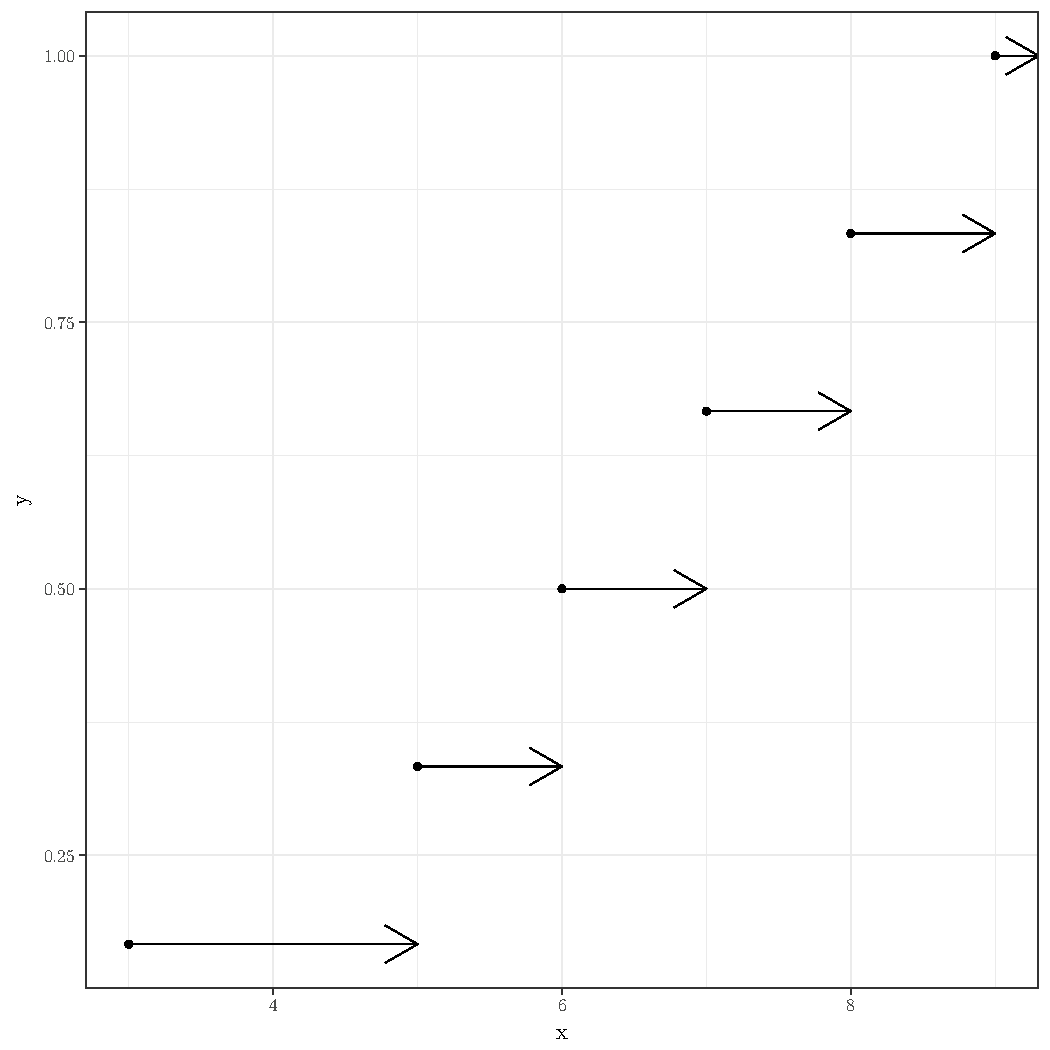
\includegraphics[scale=0.5]{auto_figures_tikz/2012_2013_fig_02_empirical_dist.pdf}
\end{center}
\end{minipage}
\end{enumerate}
